\documentclass[12pt, a4paper]{article}
\usepackage{amsmath, amssymb, mathrsfs}
\usepackage{graphicx}
\usepackage{url}
\usepackage{natbib}
\usepackage[margin=1in]{geometry}
\usepackage{braket}
\usepackage{bm}
\usepackage{tikz}
\usetikzlibrary{arrows.meta, decorations.pathmorphing, shapes.geometric}

% Journal formatting
\usepackage[colorlinks=true, citecolor=blue, linkcolor=red]{hyperref}
\usepackage{abstract}
\renewcommand{\abstractnamefont}{\normalfont\bfseries\large}
\renewcommand{\abstracttextfont}{\normalfont}

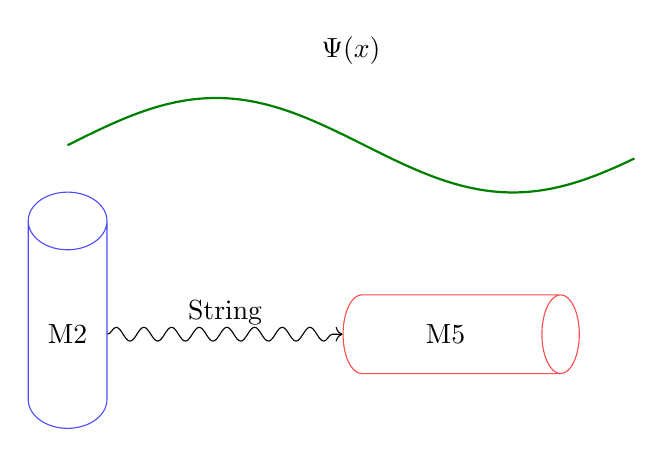
\begin{tikzpicture}[scale=1.2]
% M2 and M5 branes
\node[cylinder, draw=blue!70, minimum height=3cm, minimum width=1cm, shape border rotate=90] (M2) at (0,0) {M2};
\node[cylinder, draw=red!70, minimum height=3cm, minimum width=1cm, shape border rotate=0] (M5) at (4,0) {M5};
\draw[->, decorate, decoration={snake}] (M2) -- (M5) node[midway, above] {String};
% Coherence field
\draw[green!50!black, domain=0:6, samples=100, thick] plot (\x, {0.5*sin(\x r) + 2});
\node at (3,3) {\(\Psi(x)\)};
\end{tikzpicture}
\end{document}
